\documentclass[../SustainableHEP.tex]{subfiles}
\graphicspath{{\subfix{Sections/Figs/}}}
\begin{document}
\RaggedRight
\sloppy
\newpage

%%%%%%%%%%%%%%%%%%%%%%%%%%%%%%%%%%%%%%%%%%%%%%%%%%

\section{Computing}
\label{sec:Computing}

%%%%%%%%%%%%%%%%%%%%%%%%%%%%%%%%%%%%%%%%%%%%%%%%%%

\begin{figure}
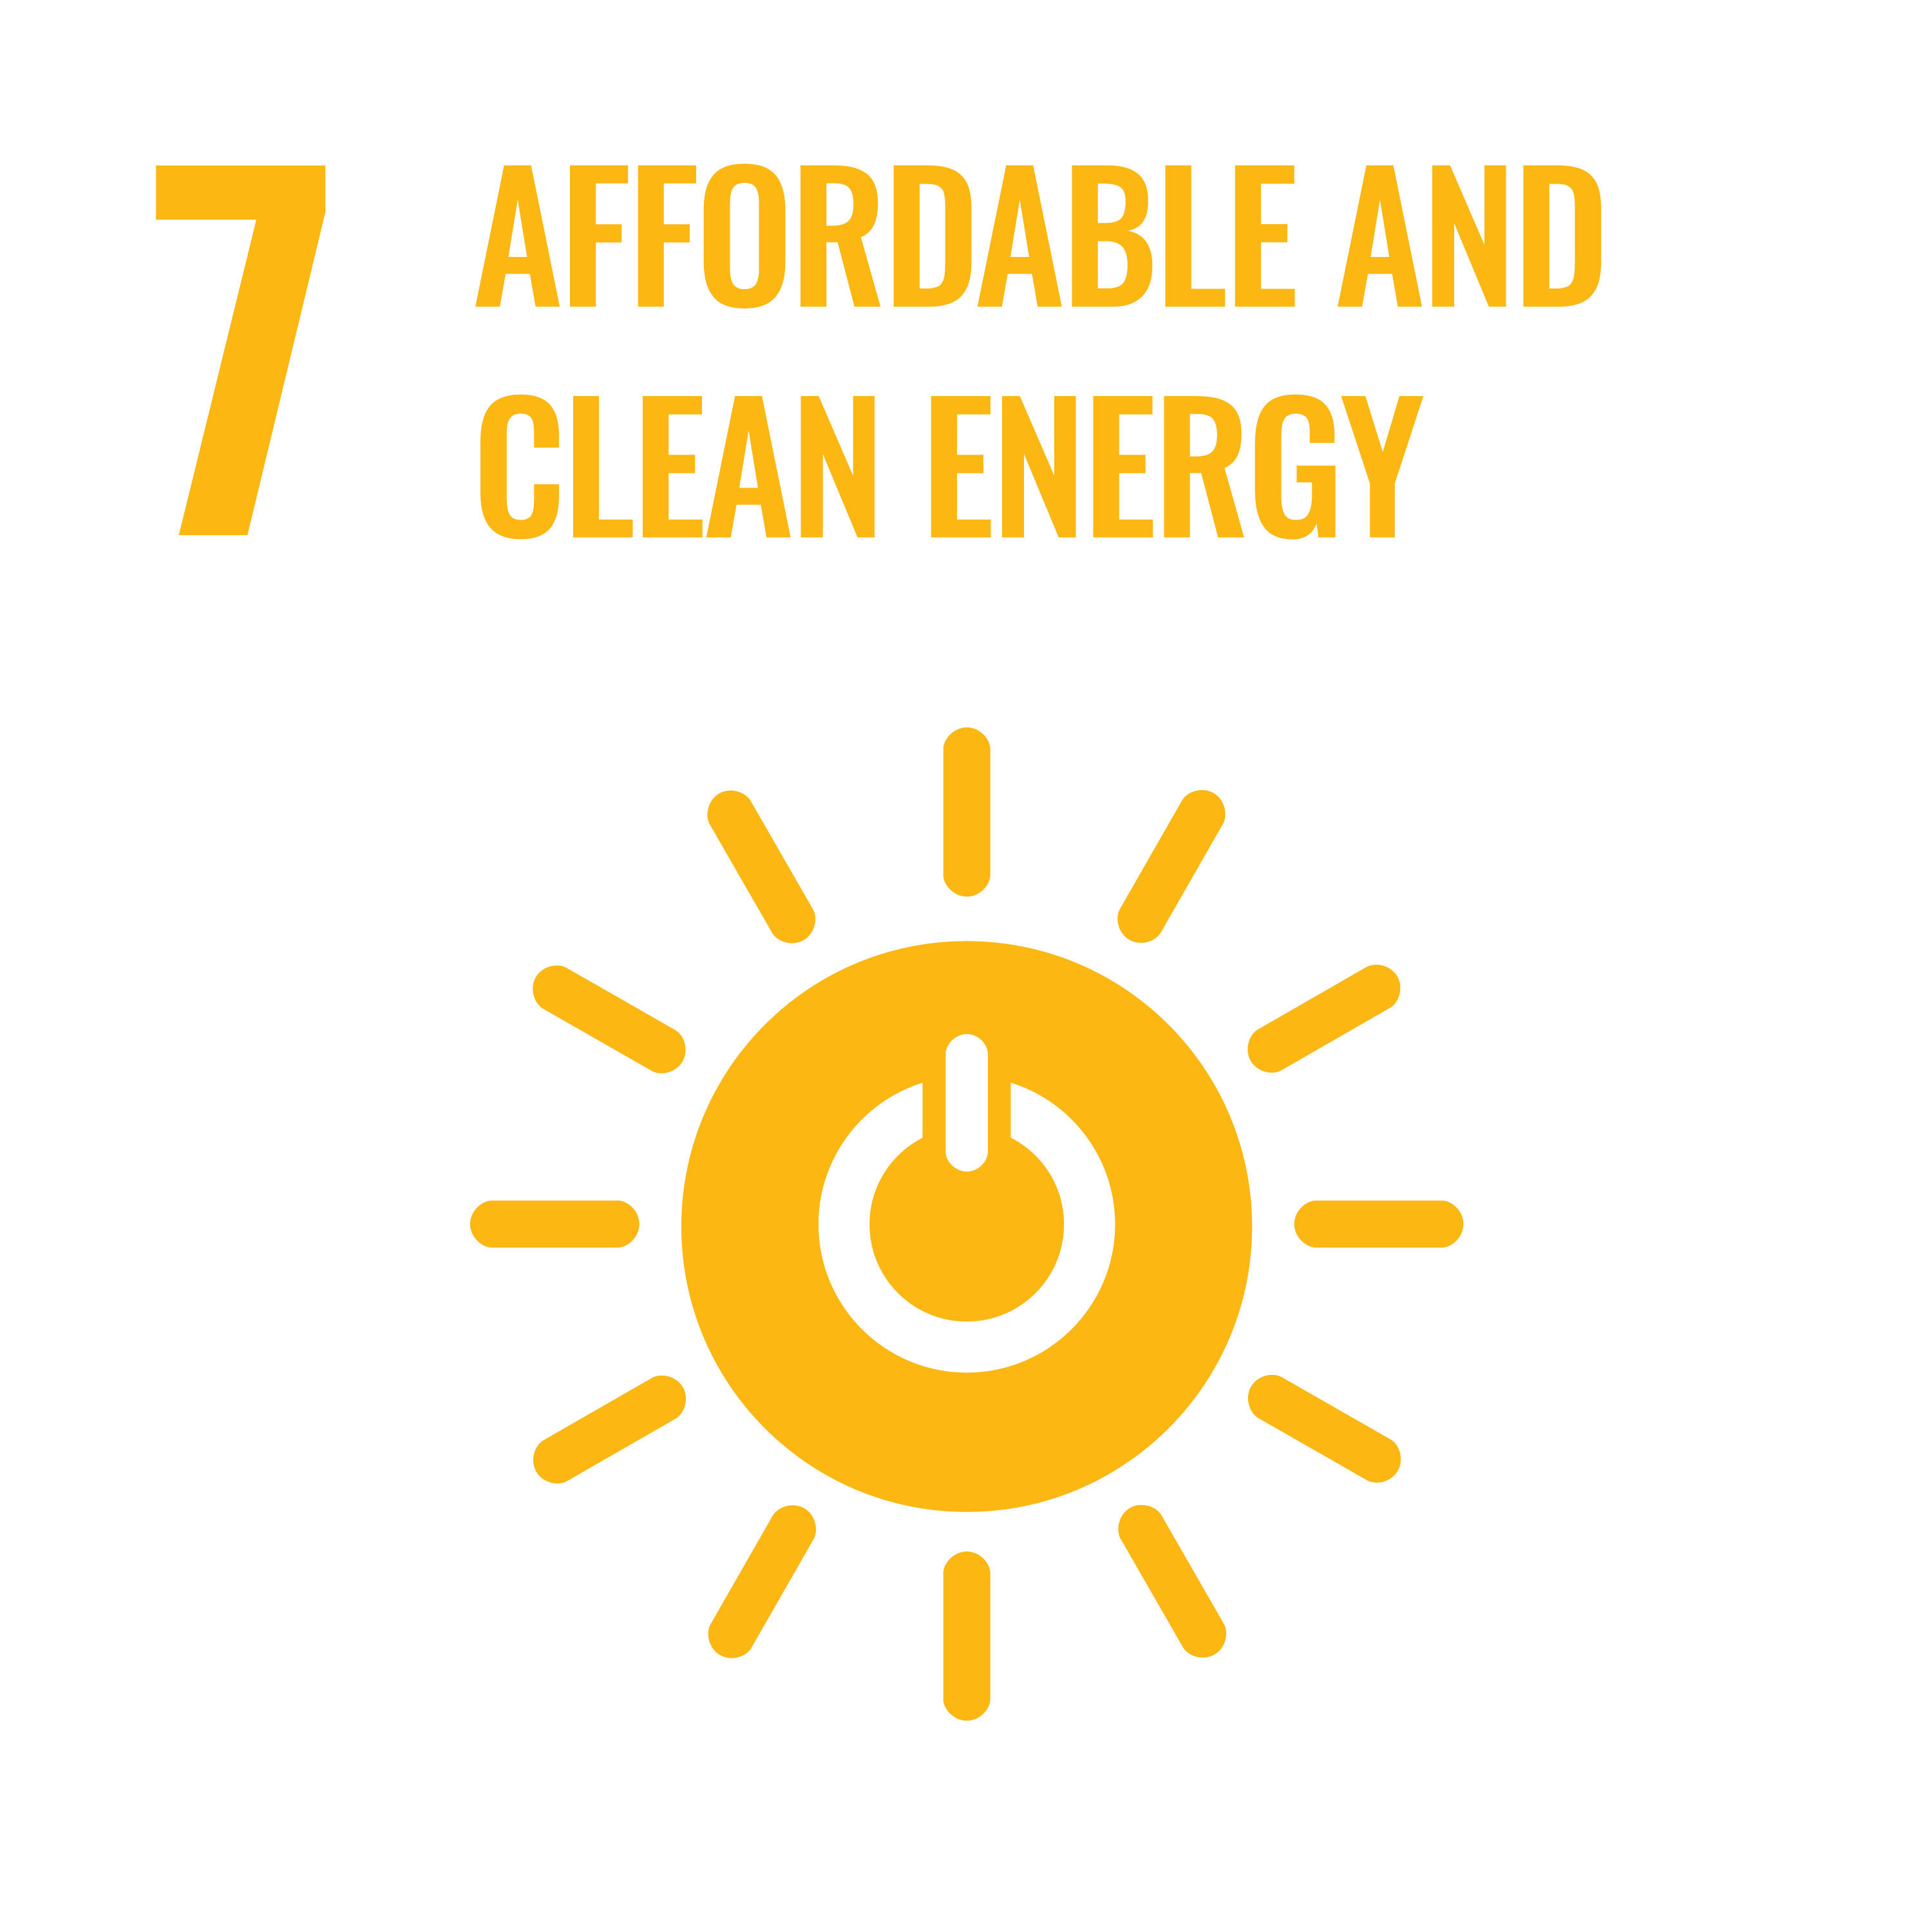
\includegraphics[width=\SDGsize]{Common/SDG_7_CleanEnergy.png}~%

\includegraphics[width=\SDGsize]{Common/SDG_9_IndustryInnovation.png}~%

\includegraphics[width=\SDGsize]{Common/SDG_12_ResponsibleConsumption.png}~%

\includegraphics[width=\SDGsize]{Common/SDG_13_ClimateAction.png}
\end{figure}

%%%%%%%%%%%%%%%%%%%%%%%%%%%%%%%%%%%%%%%%%%%%%%%%%%

\exSum

\noindent Computing represents an integral part of basic research, being used for theoretical modelling, simulation (including lattice simulation), and data analysis. With increasing data sets and demands for accuracy, computing resource consumption is expected to rise. 
This poses concerns in the context of climate sustainability. 
Within \ACR, \eg the High-Luminosity phase of the Large Hadron Collider (\acrshort{hl-lhc}), predicted to be operational from 2026, is expected to rely on 50 to 100 times the computing capacity needed for the Large Hadron Collider (\acrshort{lhc}), with data storage requirements reaching exabytes~\cite{CERN_computing_webpage}. 
At the same time, some lattice quantum chromodynamics  (\acrshort{qcd}) calculations, applied, \eg to studying heavy quark decays and anomalous magnetic moments, can be too expensive to pursue, even if approximately 10\% of open-science super-computing in the United States is devoted to such studies~\cite{Shanahan}.
Up to 88\% of the electricity consumption of an astronomy researcher at \acrshort{mpia}, shown in \fref{fig:Intro-ComparativeEmissions}, is due to (super)computing~\cite{Jahnke2020}, and \acrshort{cern}'s (now defunct) data centre in Hungary is responsible for a third of its electricity emissions when the LHC is not running~\cite{Environment:2737239}.\footnote{The total emissions due to electricity use of a CERN researcher during LHC shutdown is about a third that of a \acrshort{fnal} researcher (see Appendix~\ref{sec:DataforFig1.4} for details). CERN, however, uses mainly the French grid with its low-carbon energy, reducing its computing carbon footprint. For further discussion, see \sref{sec:Energy}.}

\ACR\ research infrastructure ranges from local and portable computing, to high-performance computing (\acrshort{hpc}) and high-throughput computing (\acrshort{htc})\footnote{Generally, synchronization requirements of large parallel HPC applications place substantial constraints on runtime scheduling choices and use of power saving functionalities.  HTC applications, on the other hand, can be naturally run in parallel, but are constrained by memory consumption and data access and transfer.} in centralised computing centres that {---} depending on the application {---} deal with large volumes of experimental data. As an international community, we also rely on communication technologies and the ability to move these large volumes of data around the globe. The infrastructure we use to do so, comprising hardware, the data centres within which the hardware is housed, and cloud computing resources used for data storage, contributes to our community's energy consumption and the waste that our research generates.  Furthermore, the energy efficiency of hardware is ultimately limited by the efficiency of the computer programmes that run on this hardware, making the \acrshort{ghg} emissions of \ACR\ researchers dependent upon the choice of software architecture.

This chapter covers sustainability in procurement, and  extending and optimising the life-cycle of computing equipment in \sref{subsec:hardware}, choice and optimisation of software in \sref{subsec:software}, and energy savings in data centres in \sref{subsec:infrastructure}.  For a full discussion of sustainable sourcing in a broader context, as well as information on E-waste and its impact, see \sref{sec:Waste}. A brief explanation of the life-cycle analysis used to estimate the cradle-to-grave environmental impact of infrastructure and technology can be found in \sref{sec:Technology}.  For other aspects of energy use, see \sref{sec:Energy}.

\newpage
\begin{reco2}{\currentname}
{
\begin{itemize}[leftmargin=6 mm]
\item Make sustainable personal computing choices by considering the necessity of hardware upgrades, the repurposing of hardware, and the environmental credentials of suppliers and their products. 

\item Assess and improve the efficiency and portability of codes by considering, \eg the required resolutions and accuracy.

\item Assess and optimise data transmission and storage needs.

\item Follow best practice in open-access data publishing, prioritising reproducibility and limiting repeat processing.

\item Read the section on E-waste (Section~\ref{sec:Waste}).

\end{itemize}
}
{
\begin{itemize}[leftmargin=6 mm]
\item Right-size IT requirements and optimise hardware lifecycles.
\item Schedule queueing systems with environmental sustainability in mind, so as to maximise the use of renewables, accounting for the geographical location of servers/data centres.
\end{itemize}
}
{
\begin{itemize}[leftmargin=6 mm]
\item Ensure that environmental sustainability is a core consideration when designing and choosing sites for large computing infrastructure, such as data centres, including, e.g., the availability of renewables, the efficiency of cooling systems and the reuse of waste heat.

\item Proceduralise the repair, upgrade and repurposing of existing computing, the de-inventorising of personal equipment for leaving personnel or for donation, and the responsible recycling of retired hardware.

\item Select cloud computing services for their carbon emission mitigation policies.

\end{itemize}
}
\footnotetext{Some of the above recommendations are based on those made by Jan Rybizki~\cite{Rybizki}.}
\end{reco2}

%%%%%%%%%%%%%%%%%%%%%%%%%%%%%%%%%%%%%%%%%%%%%%%%%%

\newpage

\subsection{Hardware}
\label{subsec:hardware}

When considering the future of sustainability in \ACR, the hardware aspect of computing is of great concern. Hardware is both energy- and resource-consuming. The manufacture, transport, energy consumption, and disposal of each piece of hardware contribute substantially to the environmental footprint of the HPC that \ACR\ relies on to analyse large swathes of data. 

Manufacture is the largest source of hardware \acrshort{ghg} emissions, with primarily fossil-fuel-powered manufacturing chains contributing as much as 80--85\% of lifetime emissions of a personal computing device~\cite{Greenpeace_Oeko, OxfordLCA}.  Moreover, production is notoriously resource-intensive~\cite{Greenpeace_Oeko}, with the mining of the necessary metals and `conflict' minerals responsible for a number of negative environmental and social effects.  Improper disposal of substances found in computing equipment is also linked to environmental hazards and a variety of other risks.    For an in-depth discussion, see \sref{sec:Waste}.

One way to mitigate the impact due to production is by purchasing modular equipment, which allows for easy upgrades and repurposing of hardware.  In fact, the extension of hardware lifetime has been increasingly demonstrated to have major benefits over upgrading to more efficient technology.  A study by the University of Edinburgh Department for Social Responsibility and Sustainability~\cite{UniEd} found that simply using 174 computer monitors for six years instead of four saved 33 \tCdOe, which, when incorporated into standard practice, would not only reduce purchasing costs, but would result in an annual GHG savings of 380 \tCdOe.  It is also crucial that institutions be able and willing to support repairs. This applies in particular to personal equipment, \eg laptops,  which come with additional peripherals such as display, keyboard, and housing, as compared with HPC units in data centres. 

Furthermore, prioritising suppliers that implement sustainable sourcing, including recovery of secondary materials, and manufacturing methods would partially mitigate the resource burden, as would enabling circularity and appropriate E-waste recycling.  As one example, TCO certification \cite{TCO_Certified} is the world-leading sustainability certification for IT products, such as those supplied by Lenovo, Dell, or Acer. TCO-certified compliance is independently verified both pre- and post-certification. TCO certification also covers data centre products, which could be given preference over uncertified ones for cluster computing. For more information on sustainable procurement, including some hallmarks of sustainability in raw materials supply chains, see \sref{subsec:Resources}.  For further discussion of E-waste, see \sref{subsec:Waste}.

A secondary source of hardware emissions is energy consumption during its use, with the majority coming from processors, memory, and runtime of jobs.  Processor upgrades and the optimisation of memory type can greatly reduce energy consumption. See \csref{case:LHCb} for details of energy-efficient hardware purchase at LHCb.

It is important to ensure `energy proportionality' in hardware use, \ie\ that energy consumption is proportional to computing performance over the full range of applications \cite{energy-prop-computing}.    Often, hardware designed to be most efficient at maximum performance load in practice spends most of its time idle, or performing less intensive computations. This can be addressed by, \eg running jobs at high utilization rate on as few servers as possible.  

Implementing parallelisation within processors can also reduce the number of processors needed, and by replacing central processing units (CPUs) with graphics processing units (GPUs), the energy usage can be reduced.  For certain tasks relevant to \ACR\ applications, other even more specialised processors are available, such as Google's tensor processing unit (TPU)~\cite{Tensor}.  This consumes less power than its predecessors, although it suffers from poor energy proportionality: at 10\% load, it consumes almost 90\% of the power it would consume at 100\% load \cite{TensorPerformance}.

However, it should always be tested whether parallelisation does reduce the overall energy usage of a task, as an increase in energy consumption per second could counteract the benefits of reduced runtime.  Another aspect to take into consideration when implementing parallelisation is the particular application, and its requirements in terms of memory, scalability, and data access. Reference~\cite{Abdurachmanov:2014xka} discusses these issues in the context of the Worldwide Large Hadron Collider Computing Grid (WLCG).  It also gives suggestions for power-aware software applications and scheduling that could reduce power consumption.  Some of the advocated changes are software specific and are further detailed in \sref{subsec:software}. The Green500 list~\cite{GreenList} ranks the most energy efficient high-performance computing systems. 
The GHG emissions of the computer centres that house them, however, depend critically on their infrastructure. This aspect is further discussed in~\sref{subsec:infrastructure}.

%%%%%%%%%%%%%%%%%%%%%%%%%%%%%%%%%%%%%%%%%%%%%%%%%%

\subsection{Software}\label{subsec:software}

Software is integral to the work of \ACR. It underpins how the global \ACR\ community communicates, shares data, produces papers and graphics, and acquires, manages, processes and analyses huge amounts of data from experiments, observatories and simulations.

It is therefore pivotal that the software developed and used by the \ACR\ community is efficient in order to minimise CPU hours, and to facilitate data sharing and long-term reproducibility. This requires a balance to be struck between portability and optimisation for particular architectures.  While not directly linked to environmental sustainability, initiatives focused on software sustainability in \ACR, such as the \acrshort{iris-hep}~\cite{IRISHEP} and the \acrshort{hep} Software Foundation~\cite{HSF}, may provide an important platform for accelerating the inclusion of  environmental considerations in software development. Doing so is compatible with the \acrshort{fair} principles~\cite{FAIR} for scientific data management, that software (and data) should be Findable, Accessible, Interoperable and Reusable.

Much of the code used in \ACR\ computing relies on libraries and public codes. Experiments use general frameworks and software infrastructure provided by experts in the experiments. They can have a tremendous impact on the energy efficiency of the employed code and, in some cases, work to meet strict requirements posed by the computing environment. Decisions on the computing language employed can be crucial, with Fortran and C++ specifically suited for numerical calculations, whilst others prioritise convenience or readability over performance.  Changes in processor architecture have been utilised through dedicated and collaborative  efforts, leading to a factor of 2 improvement in the performance (and energy efficiency) of the reconstruction code of the \acrshort{atlas} experiment~\cite{ATL-SOFT-PUB-2021-002}. Other examples of software improvement are recent changes to the software framework and architecture at LHCb (see \csref{case:LHCb}) and improvements in a MC generator core code, having led to an improvement in speed of a factor of 50 (see \bpref{CS:SoftwareOptimisation}).  In the case of cosmological analyses, it has been suggested that the Likelihood Inference Neural Network Accelerator (LINNA) can lead to efficiency increases that would save  \$300,000 in energy costs and around 2,200 \tCdO\ in first-year Rubin Observatory's Legacy Survey of Space and Time (LSST) analyses~\cite{To:2022ubu}.

Sustainable use of software can also be encouraged at an individual level. The energy used in a job directly correlates with the memory assigned/available for a job, so mitigation by individuals can be easily implemented through assigning the correct memory used and by optimising code~\cite{Karayakin}. Further examples of conscientious use of software include limiting resolution or precision to that which is necessary, effective testing to avoid wasted CPU hours, good practice in data retention to avoid data loss and the need to rerun analysis or simulations, and scheduling CPU hours when a higher percentage of the local energy mix is from renewables.

\begin{bestpractice}[Optimization of software\label{CS:SoftwareOptimisation}]{Optimization of software}%
A targeted effort enabled by the UK-based SoftWare and InFrastructure Technology for High Energy Physics (\acrshort{swift-hep})~\cite{SWIFTHEP} project recently brought together experimentalists and Monte Carlo (\acrshort{mc}) developers to greatly improve the computational efficiency of multi-leg next to leading order (\acrshort{nlo}) calculations by focussing on two major components of general purpose MC event generators: The evaluation of parton-distribution functions (\acrshort{pdf}s) along with the generation of perturbative matrix elements. A dedicated CPU profiling illustrated that for the cost-driving event samples employed by the ATLAS experiment to model irreducible Standard Model backgrounds, such as V+jets as well as ttbar+jets production, these components dominate the overall run time by up to 80\%. Improved interpolation and caching strategies in LHAPDF \cite{Buckley:2014ana}, the main evaluation tool for PDFs used by the experiments, along with the introduction of a simplified pilot run in the MC generator Sherpa~\cite{Sherpa} for the unweighting achieves a reduction of the computing footprint by factors of around 50 for multi-leg NLO event generation, while maintaining the formal accuracy of the event sample~\cite{Bothmann:2022thx}. The speed-up translates into a direct CPU (and hence energy) saving, paving the way towards affordable and sustainable state-of-the-art event simulation in the HL-LHC era.

\end{bestpractice}

%%%%%%%%%%%%%%%%%%%%%%%%%%%%%%%%%%%%%%%%%%%%%%%%%%

\subsection{Infrastructure}\label{subsec:infrastructure}

Even the most energy-efficient data centres are not environmentally sustainable if they are powered by carbon-based fuels~\cite{Bloom:2022gux}.  
However, provided energy from renewable sources is available, this can be easily addressed. Indeed, there are many advantages to doing so, owing to the flexibility of HTC.
Inherent fluctuations in supply of electricity from renewables can be managed using a smart queueing system that runs jobs at times where electricity has a large renewable component,
 or directs them to data centres where this is the case.  
Moreover, a carefully-managed HTC system can even help stabilise fully-renewable power grids in response to local imbalances in supply and demand: 
an instantaneous reduction in the CPU clock frequency by up to 60\% ensures per-second grid stabilisation,
and a similar technique can be employed on longer time scales, \eg hourly, in response to changes in the carbon intensity of electricity (or equivalently, market price). 
For longer periods, with higher latency, this can also involve powering down nodes. 
The reduced work can be compensated by operating older hardware longer, but only when the electricity price is low.  
See \sref{sec:Ene-Transition} for further discussion of renewables-based grid infrastructure.  

Another source of GHG emissions associated with computing is the construction and operation of the large data centres within which IT equipment is housed.  Although emissions due to construction can be significant, particularly if concrete is used, our focus in the remainder of the section will be on cooling the facilities and equipment, which is responsible, on average, for almost one third of facility power use. A judicious choice of location for the centre can minimise these energy costs, by provision of a cooler external environment, or other means to cool efficiently.  Proximity to a large body of water, \eg could make water cooling an attractive option.  Care must be taken, however, to ensure minimal disruption to the natural environment.  Waste heat from the data centre can also be reused to heat nearby infrastructure. For examples of best practice in data centre design and construction, see \bpref{BP:CSCS}, \bpref{BP:Prevessin}, and \bpref{BP:GreenITCube}.  For more information on energy-efficient LHCb computing infrastructure, see \csref{case:LHCb}. 

%%%%%

\begin{bestpractice}[\label{BP:CSCS}Cooling in Swiss National Supercomputing Centre\\
{\footnotesize \noindent Information taken from CSCS fact sheets \cite{CSCSLakeWater,CSCSInnovativeBuilding} and vetted by the organization.}]{Cooling in Swiss National Supercomputing Centre (CSCS)}%
    The Swiss National Supercomputing Centre (\acrshort{cscs}) is a three-floor concrete building in Lugano that houses the “Piz Daint” supercomputer and the system used by MeteoSwiss for weather predictions, among other things.  It currently operates at a \acrshort{pue} rating of 1.20 at 25\% of full load, with a design PUE of 1.25.\footnote{PUE measures the overhead energy costs of an IT facility, and is defined as the ratio of the total power used by the facility over the energy used by the IT equipment.}
    At CSCS, high-efficiency cooling is achieved with a state-of-the art cooling system using the water from Lake Lugano, extracted at a depth of 45 m 
    and a temperature of 6\degree C. 420 litres of this water per second are pumped to the facility over a distance of 2.8 km into large heat exchangers, where it meets and cools the water in the internal cooling circuit for the supercomputers. The resulting warmer water is then sent to a heat exchanger in a second cooling circuit, which cools the components with a lower thermal sensitivity, as well as the building itself in the summer, before being returned to the lake. The return flow of water falling back into the lake is used to produce electricity via a microturbine in the pumping station further reducing the power consumption of the pumps by 30\%.  Due to modular cooling and room concepts, the different parts of the facility are equipped only as necessary.  Not only does this reduce the initial budgetary outlay, but it also results in increased flexibility to react to future hardware needs, while keeping the PUE close to its final design value from the outset.
\end{bestpractice}

\begin{bestpractice}[\label{BP:Prevessin}Sustainable design for Prevessin Computing Centre, CERN\\{\footnotesize \noindent Contribution by Wayne Salter, IT Project Manager for the PCC}]{Sustainable design for Prevessin Computing Centre, CERN}%
CERN has for some time been wishing to build a second Data Centre (\acrshort{dc}) on its Pr\'{e}vessin site (named the \acrshort{pcc}) to augment the capacity being provided by its Meyrin Data Centre, in particular in light of the increased demands from the LHC experiments in the HL-LHC era.
In 2019, a project was approved to build a turn-key Data Centre (\acrshort{dc}) with an initial capacity for computing of 4 MW, but with the possibility to upgrade the IT capacity in two steps to 8 MW and finally to 12 MW. 
A Call for Tender was initiated at the end of 2019 for the design, construction and 10 year operation and
maintenance of a new \acrshort{dc} and the result of the tender was
adjudicated at the CERN Finance Committee in December 2020 in favour of a consortium led by EQUANS~\cite{EQUANS}. A contract was signed with the winning
consortium in July 2021 and construction began at the beginning of 2022.
The DC is expected to be operational in the final quarter of 2023. An
important aspect included in the thinking for the new DC was
sustainability and, in particular, energy efficiency. As such, the
specification required a target Power Usage Effectiveness (\acrshort{pue}) of 1.1,
but contractually allows for a \acrshort{pue} of no worse than 1.15, for energy
recuperation of at least 25\% of the heat generated by the IT equipment
and for a roof with vegetation.

When considering the increased energy efficiency compared with CERN's
existing Meyrin Data Centre, which now has a PUE of around 1.5 after
many years of efforts to bring this down, this equates to significant
energy savings. Assuming the PCC running at full first phase capacity of
4 MW with a PUE of 1.1, cf.~1.5 for the current CERN Data Centre, then
the annual saving in terms of electricity would be 14 GWh. Obviously,
should the PCC be eventually upgraded and used at its full final
capacity then the savings could be tripled, cf.~with running a similar
capacity with the PUE of the current Meyrin Data Centre. It should be
noted that the PUE of the current Data Centre is the result of many
years of efforts to improve the energy efficiency, which have
substantially reduced its PUE, but that further improvements would now
be complex and costly.

In addition to aiming for high energy efficiency, the design of the PCC
also allows for the heat produced by the IT equipment to be recuperated
and used to help power a new building heating plant that will soon be
built close to the PCC to replace an existing ageing and inefficient
heating plant. 
The specification for the PCC required the possibility
to recover a minimum of 25\% of the generated heat per phase, implying
1.3 MW per phase leading to a total of 3 MW once the full 12 MW
configuration would be operational. However, during the design phase it
has been decided to request 3 MW already during the first phase. In the
second phase, the heat recuperation will be increased to 4 MW.

During hot weather, water is sprayed on the heat exchanger elements of
the dry coolers to improve their efficiency. In the original design, this
water was lost, resulting in a non-insignificant water consumption over
the year. However, with sustainability and environmental protection
considerations in mind, it was decided to make efforts to reduce the
water consumption as far as possible without impacting the efficiency of
the cooling solution. As such, it was agreed with the contractor to
change the design to include water re-circulation at the level of the dry
coolers and hence substantially to reduce the water consumption. In the
first phase, the annual water consumption is estimated to be reduced by 61\% from
21,455 ${\rm m}^3$ to 8,645 ${\rm m}^3$, based on the average meteorological data for the area.

To further improve sustainability and to make the building more
ecologically friendly, it was also decided to request that vegetation be
planted on the roof of the building, which is effectively in two halves.
The first half contains the IT rooms (two per floor for three floors) and
the second half is for all the technical rooms. The roof is similarly
split in two. The first half is used for the dry coolers and associated
technical infrastructure and hence cannot be used for vegetation, but
the second half will be planted with grass covering an area of
approximately 1,250 ${\rm m}^2$.
\end{bestpractice}

\begin{bestpractice}[\label{BP:GreenITCube}The Green-IT Cube at GSI/ FAIR~\cite{GreenITCube}]{Green-IT Cube}%
\noindent At  GSI Helmholtzzentrum für Schwerionenforschung in Darmstadt, the Green-IT Cube~\cite{GreenITCube} was constructed in 2014 to host the computing systems of the FAIR facility under construction close to GSI, as well as numerous other scientific computing systems. It has a total capacity of 12 MW and 768 racks, distributed over 6 floors. The partial \acrshort{pue}, that is the PUE across some part of the data centre, see, Sec. VII of Ref.~\cite{GreenGridPUE}) of the installation reaches 1.07 at a load of <25\%, which meets the design value. In acceptance testing at higher loads an even better partial PUE has been observed.
 
This became possible due to the award-winning innovative design of the Green-IT Cube, which was developed at the Frankfurt Institute of Advanced Studies by Volker Lindenstruth. The innovative design based on water cooled back-door heat exchangers allowed not only for a low PUE, but also for an advanced 3D building design which reduced the ground print of the compact data center. At the same time it reduced the building material needed, further reducing the environmental impact. Parts of the excess heat are used to heat office buildings on the GSI campus.
 
The patented design has received many innovation and data center awards and was successfully transferred into industry.
\end{bestpractice}

%%%%%

\end{document}